\documentclass[conference]{IEEEtran}
\usepackage{amsmath,amssymb}
\usepackage{graphicx}
\usepackage{booktabs}
\usepackage{array}
\usepackage{stfloats}
\usepackage{cite}
\usepackage[hidelinks]{hyperref}
\graphicspath{{figures/}}
\renewcommand{\arraystretch}{1.12}
\renewcommand{\topfraction}{0.9}
\renewcommand{\dbltopfraction}{0.9}
\renewcommand{\textfraction}{0.07}
\renewcommand{\floatpagefraction}{0.85}
\renewcommand{\dblfloatpagefraction}{0.85}
\setcounter{topnumber}{3}
\setcounter{dbltopnumber}{2}

\usepackage{etoolbox}
\makeatletter
\newcommand{\nodashpatch}[1]{%
  \patchcmd{#1}{\textit{\abstractname}---}{\textit{\abstractname}:\ }{}{}%
  \patchcmd{#1}{\textit{\abstractname}---}{\textit{\abstractname}:\ }{}{}%
  \patchcmd{#1}{\textbf{\abstractname}---}{\textbf{\abstractname}:\ }{}{}%
  \patchcmd{#1}{\textit{\IEEEkeywordsname}---}{\textit{\IEEEkeywordsname}:\ }{}{}%
  \patchcmd{#1}{\textit{\IEEEkeywordsname}---}{\textit{\IEEEkeywordsname}:\ }{}{}%
  \patchcmd{#1}{\textbf{\IEEEkeywordsname}---}{\textbf{\IEEEkeywordsname}:\ }{}{}}
\nodashpatch{\abstract}\nodashpatch{\IEEEkeywords}
\makeatother

\begin{document}

\title{Statistical Modelling of Packet-Loss Patterns in Computer Networks: Distribution Fitting, Burstiness Testing and Bayesian Estimation}

\author{\IEEEauthorblockN{Kyra Panwar}\IEEEauthorblockA{VIT Vellore\\25BBS0095}
\and
\IEEEauthorblockN{Shashank Tiwari}\IEEEauthorblockA{VIT Vellore\\25BDS0053}
\and
\IEEEauthorblockN{Aashman Biyani}\IEEEauthorblockA{VIT Vellore\\25BBS0100}}

\maketitle

\begin{abstract}
Simplest models treat each lost packet as independent of the others which is why most of the times a single number is reported as the loss rate. If this was true, the number of losses in each second would follow a Poisson distribution whereas the gaps between consecutive losses would follow an exponential distribution model. Three networks (wired broadband, campus Wi-Fi and a mobile hotspot) were simulated with a two-state Gilbert-Elliott model, each sending <<rate>> packets per second for <<duration_h>> hour, which comes to <<packets>> packets per network. We fitted models for the counts and for the waiting times, tested whether neighbouring packets are independent, and estimated the loss rates with a Bayesian Beta-Binomial model. Independence did not hold on any of the <<n_scen>> networks. The variance of the per-second loss count was <<list_D>> times the mean, where a Poisson model gives 1, and after a single loss the next packet was <<amp_lo>> to <<amp_hi>> times more likely to be lost. This shows up directly in the error bars. Over <<cov_reps>> simulated captures, the standard 95\% interval for the loss rate contained the true value in only <<covN_lo>> to <<covN_hi>> of cases. Reducing the sample size by a design effect raised coverage to between <<covA_lo>> and <<covA_hi>>. A power study suggests recording at least ten minutes on each network once we move on to real measurements.
\end{abstract}

\begin{IEEEkeywords}
Packet loss, Gilbert-Elliott channel, overdispersion, goodness of fit, Bayesian estimation, design effect, Monte Carlo.
\end{IEEEkeywords}

\section{Introduction}
Packet loss is a common issue faced by almost everyone at a certain point in their lives unknowingly. For example, a student attending an online class might have to face audio disruptions and video interruptions. The reason behind this is that packets, which are units of data during transmission, are unable to reach their destination. Applications send packets at a fixed rate and the proportion of the packets that are lost during transmission is known as the packet loss rate. This criterion has an important role in evaluating network performance as it is used to define acceptable level of service quality in service level agreements, helps communication protocols to decide retransmission timers, and also determine the level of error correction needed by a stream.

However, the loss rate cannot depict how the losses are distributed over a period of time. If 10 packets are lost in a scattered manner the decoder is able to hide them and these losses go unnoticed by the user, but a cluster of 10 packet losses will cause an obvious freeze. From our data, the worst single second lost 7 out of 50 on wired, 25 on Wi-Fi, and 40 on mobile connection while most seconds lost none of the packets. Textbooks generally assume that each packet is lost independently with a probability $p$. This would suggest that packet losses occur in a binomial, or almost Poisson, distribution and at the same time the gaps in between consecutive packet losses would be exponential. But on comparing with simulations and subsequent results it is found that these distributions do not actually follow the obtained data once the losses start to cluster.

Our aim was to find out how badly independence fails, which standard tests pick up the failure, and what it does to the interval estimates usually reported for the loss rate. The work is split into two phases, and this report covers Phase 1, a simulation study. Because we set the true parameters of each network ourselves, we can compare every estimate and test with the correct answer before the same code is used on real data. Phase 2 will apply that code to real captures.

The report is organised as follows. Section~II gives some background, Section~III sets out the loss model and how the data were generated, Section~IV describes the statistical methods and Section~V reports the results. Section~VI discusses what the results mean and where the study is limited, and Section~VII concludes.

\section{Background}
Modelling bursty errors with a hidden two-state chain goes back to E.~N.~Gilbert, who used it for errors on telephone lines in 1960 \cite{gilbert1960}. In 1963 E.~O.~Elliott extended the model so that errors could occur in either state \cite{elliott1963}. The Gilbert-Elliott model that came out of this is still the usual starting point for bursty loss.

It has also been known for many years that Internet losses are not independent. Measurement studies in the 1990s showed that probe packets sent close together were often lost together \cite{bolot1993}, and that losses in TCP transfers came in correlated episodes \cite{paxson1997}. The timing of loss in multicast traces could be described reasonably well with Markov chains \cite{yajnik1999}. Later studies fitted Gilbert models to voice traffic and related the length of a loss burst to how poor a call sounds \cite{jiang2000,hasslinger2008}.

Most of this earlier work sets out to describe the loss process. Our interest is more statistical. We want to know which standard tests detect the dependence, how much data they need before they do, and how far ordinary interval estimates drift from the truth when the dependence is ignored. For the last of these we use the design effect from survey sampling \cite{kish1965}, where it corrects for people being sampled in clusters instead of one at a time.

\section{Loss Model and Data}
\subsection{The Gilbert-Elliott Channel}
We treat the network as being in one of two hidden states, Good (G) or Bad (B). We cannot observe the state itself, only what it does to the packets. Before each packet, the channel switches from Good to Bad with probability $p$ and from Bad back to Good with probability $r$. In the Good state a packet is lost with a small probability $h_G$; in the Bad state the probability $h_B$ is much larger. Over a long run, the flow into the Bad state has to equal the flow out of it. This gives the share of time spent in Bad, and from it the overall loss rate:
\begin{equation}
\pi_B=\frac{p}{p+r},\qquad P(\text{loss})=(1-\pi_B)\,h_G+\pi_B\,h_B .
\label{eq:ge}
\end{equation}
The number of packets spent in a state before leaving it is geometric, with a mean of $1/p$ packets for Good and $1/r$ for Bad. A burst of losses happens whenever the channel drops into the Bad state for a few packets.

\subsection{Scenarios and Sampling}
Table~\ref{tab:params} summarizes the parameters for the three networks, namely, wired, Wi-Fi and mobile connections with low, medium and high loss respectively. Each network spends 0.17\%, 1.32\% and 4.76\% of the time in the Bad state. This is done so that networks with higher loss rates spend more time in Bad state. Close to the rate of a voice call, every network sends 50 packets per second. The simulation lasts for 3600 seconds and produces a total of 180,000 packets per network. All the random numbers were taken from seed 2026, so anybody who reruns the simulation will obtain the exact same numbers.

\begin{table}[!t]
\caption{Scenario parameters and the true loss rate they imply}
\label{tab:params}
\centering
\footnotesize
\setlength{\tabcolsep}{3.2pt}
\begin{tabular}{lccccccc}
\toprule
Network & $p$ & $r$ & $h_G$ & $h_B$ & $\pi_B$ & Bad spell & True loss \\
\midrule
<<rows_params>>
\bottomrule
\end{tabular}
\\[2pt]
\raggedright\scriptsize Bad spell is the average stay in the Bad state, $1/r$ packets. True loss comes from (\ref{eq:ge}).
\end{table}

\subsection{Simulation}
The order can be simulated by going packet by packet which is correct, but it is also slow. Rather, we take each Good spell and Bad spell straight from the geometric distribution and lay them end to end, which is a far faster method of going about this. Then, for every packet, we decide whether it is lost using the loss probability of the state it falls in. The process is the same, just far quicker to generate. We take four things from each trace: the number of losses in each <<window_s>>-s window (<<windows>> counts per network), the gaps between successive losses, the lengths of bursts (runs of consecutive losses), and how often a delivered (N) or lost (L) packet is followed by each type of packet. Fig.~\ref{fig:timeline} plots the first few minutes of each trace. On Wi-Fi and the mobile hotspot the clumping can already be seen by eye.

\begin{figure}[!t]
\centering
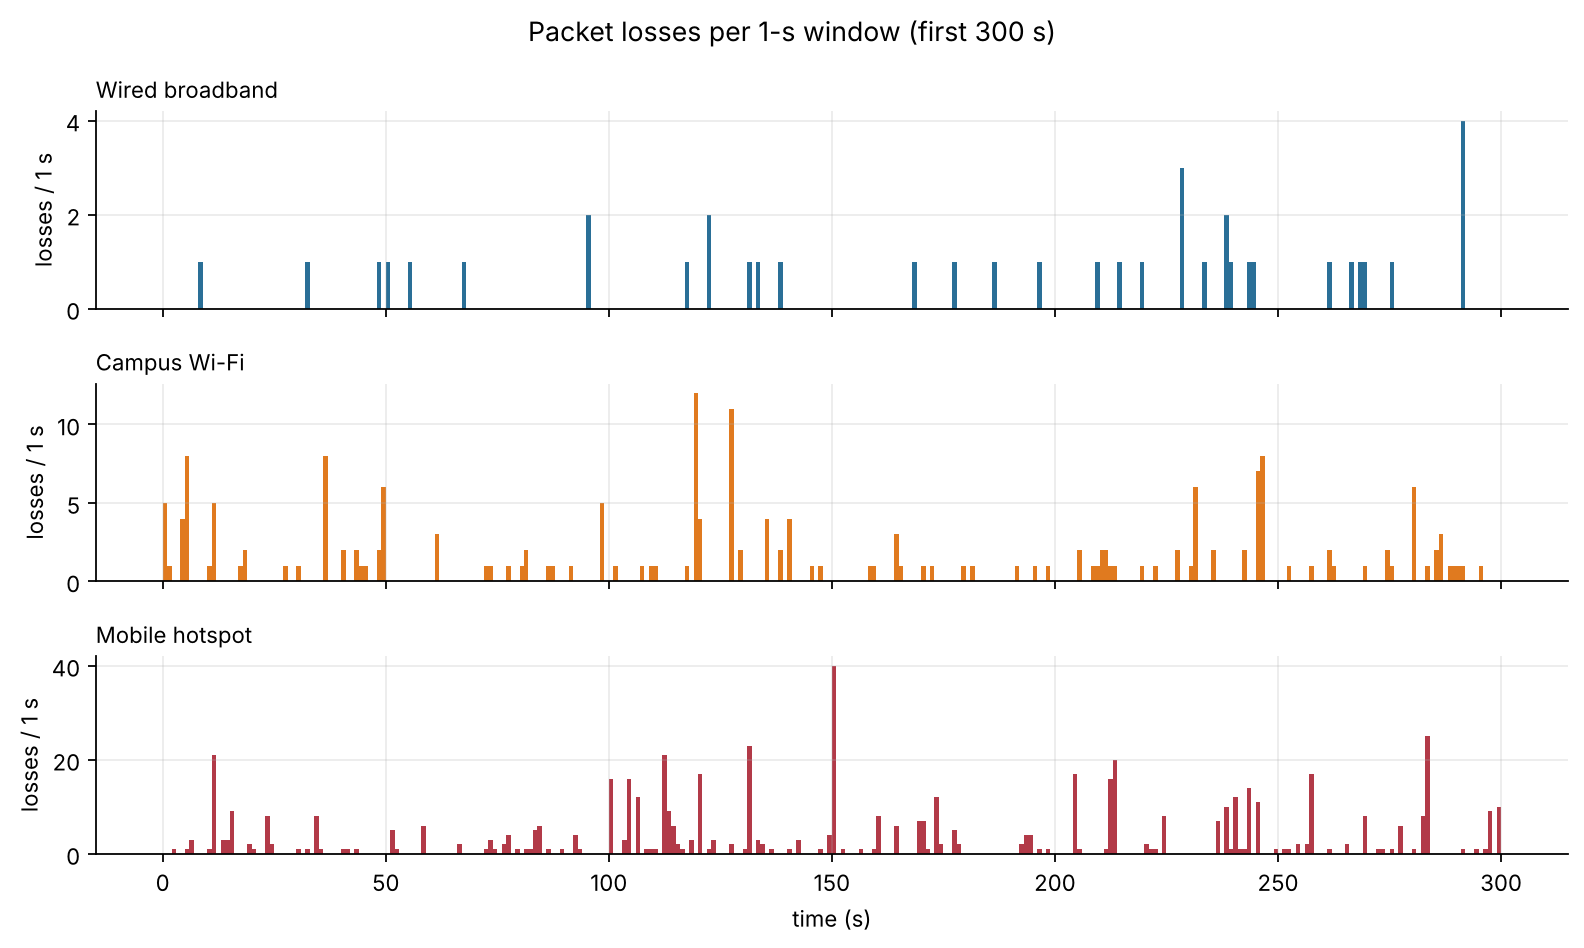
\includegraphics[width=\columnwidth]{fig1_loss_timeline.png}
\caption{Losses per second during the first five minutes of each simulated trace. On Wi-Fi and the mobile hotspot the losses come in clusters instead of one at a time.}
\label{fig:timeline}
\end{figure}

\section{Methodology}
\subsection{Fitting the Distributions}
For the per-window loss counts $x_1,\dots,x_n$, the first model we fit is the Poisson distribution, whose maximum-likelihood estimate is simply the mean count, $\hat\lambda=\bar x$. The natural alternative is the Negative Binomial:
\begin{align}
P(X=k)&=\binom{k+r_{\!NB}-1}{k}q^{r_{\!NB}}(1-q)^k,\\
\operatorname{Var}(X)&=\mu+\mu^2/r_{\!NB} .
\end{align}
The Negative Binomial can be thought of as a Poisson whose rate changes over time, which is what a network moving between good and bad periods produces. The extra term $\mu^2/r_{\!NB}$ lets the variance exceed the mean, something the Poisson cannot do. We fit it by fixing the mean at $\bar x$ and searching for the $r_{\!NB}$ that maximises the likelihood.

For the gaps between losses we begin with the exponential distribution, with $\hat\lambda=1/\bar t$, and compare it with a mixture of two exponentials known as the two-phase hyperexponential:
\begin{equation}
f(t)=w\lambda_1e^{-\lambda_1t}+(1-w)\lambda_2e^{-\lambda_2t}.
\end{equation}
The idea behind the mixture is that gaps come in two types. Short gaps, with the fast rate $\lambda_1$, occur within a burst. Long gaps, with the slow rate $\lambda_2$, occur between bursts. We never know which type a particular gap is, so we fit the mixture with the Expectation-Maximisation (EM) algorithm \cite{dempster1977}. In each iteration the E-step works out the probability that each gap is a short one, and the M-step updates $w$, $\lambda_1$ and $\lambda_2$ with these probabilities as weights. We stop once the fit no longer improves. Models are compared with the Akaike Information Criterion, $\text{AIC}=2k-2\ln L$ \cite{akaike1974}. It rewards a good fit but adds a penalty for each extra parameter, so a lower value means a better model.

\subsection{Goodness of Fit}
We evaluate the goodness of fit by comparing the observed and expected number of seconds with $k$ losses under each model using the Pearson statistic $\chi^2=\sum_i (O_i-E_i)^2/E_i$. The test is unreliable when expected counts in the tail are small, so tail bins are merged until every expected count is at least 5. The degrees of freedom are the number of bins, minus one, minus the number of fitted parameters. We also check the Poisson assumption by using the index-of-dispersion test. In a Poisson distribution, the variance equals the mean. The test statistic is $(n-1)s^2/\bar x$ and follows a $\chi^2_{n-1}$ distribution. A variance which is greater than the mean indicates overdispersion and produces a large statistic value.

For the gaps between losses, the goodness of fit is assessed using the Kolmogorov-Smirnov (KS) distance test $D=\sup_t|F_n(t)-F(t)|$, which measures the maximum difference between the data curve and the model curve. One complication is that the standard KS tables assume the model was fixed before the data were seen. Here the rate is estimated from the same data, which makes the fit look better than it is and leaves the textbook p-value too large \cite{lilliefors1969}. Parametric bootstrap is used to get the p-value instead \cite{efron1993}. Synthetic datasets are generated from the fitted model, the model parameters are re-estimated and the $D$ value is recomputed. This procedure is conducted 2,000 times for the exponential and 500 times for the mixture models because the Expectation-Maximisation (EM) refit is rather slow. This gives the range of $D$ to expect if the model is correct.

\subsection{Testing Independence}
A run is a sequence of same outcomes. For example, 0\,0\,1\,1\,0\,0\,0 has 3 runs. The Wald-Wolfowitz runs test \cite{wald1940} works exactly like this and counts the number of runs $R$. With $n_1$ losses and $n_0$ deliveries, independence gives
\begin{equation}
E[R]=\frac{2n_1n_0}{n}+1,\quad \operatorname{Var}(R)=\frac{2n_1n_0(2n_1n_0-n)}{n^2(n-1)} .
\end{equation}
When losses tend to occur together, the sequence switches between lost and delivered less often than it would by chance, and $R$ ends up smaller than expected.

The Markov-chain test asks the question more directly: does the outcome for one packet depend on the packet before it? Under $H_0$ all packets share a single loss probability. Under $H_1$ there are two, $a=P(L\mid N)$ after a delivered packet and $b=P(L\mid L)$ after a lost one. Writing $n_{xy}$ for the number of times outcome $x$ is followed by outcome $y$,
\begin{equation}
\hat a=\frac{n_{NL}}{n_{NN}+n_{NL}},\qquad \hat b=\frac{n_{LL}}{n_{LN}+n_{LL}},
\end{equation}
\begin{equation}
G^2=2(\ln L_1-\ln L_0).
\end{equation}
Because $H_1$ has one parameter more than $H_0$, Wilks' theorem \cite{wilks1938} says that $G^2$ is approximately $\chi^2_1$ when $H_0$ holds. The two estimates are useful on their own as well. The ratio $b/a$ measures how much a loss raises the chance of the next loss, and $1/(1-b)$ gives the mean burst length.

The three networks are compared with rank-based tests, since the counts are mostly zero, strongly skewed and far from normal. The Kruskal-Wallis test \cite{kruskal1952} compares all three networks together. To ensure that running three tests at a time does not raise the false-alarm rate, pairwise Mann-Whitney tests \cite{mann1947} are used to compare 3 pairs using a Bonferroni correction. A chi-square test of homogeneity on total lost and delivered packets checks whether all the networks have the same loss proportion or not. All tests use $\alpha=<<alpha>>$.

\subsection{Bayesian Estimation}
We calculate the loss rate in the Bayesian manner \cite{gelman2013}. The prior used is flat, specifically $\text{Beta}(1,1)$, and this assumes that all possible loss rates between 0 and 1 are equally likely prior to any data being observed. Once $k$ losses have been observed among $n$ packets, the posterior distribution becomes $\text{Beta}(1+k,\,1+n-k)$, which means that updating the estimate simply requires adding the number of observed losses and deliveries to the initial counts in the prior. We give the mean of the posterior together with its 95\% credible interval, and in the case of Campus Wi-Fi we also illustrate how the posterior becomes narrower as more traffic is observed. To verify that the networks actually are arranged in order of loss rate, we take 200,000 samples from each posterior and then determine the proportion of those samples for which Wired $<$ Wi-Fi $<$ Mobile.

The way in which the burst parameters are treated is the same. We place separate posteriors on $a$ and $b$, $a\sim\text{Beta}(1+n_{NL},1+n_{NN})$ and $b\sim\text{Beta}(1+n_{LL},1+n_{LN})$, and these give credible intervals for $b/a$ and for the burst length. To check the independent model, we use it to predict how frequently a window should contain at least five losses and then compare that frequency with the actual frequency at which it occurs.

\subsection{Design Effect}
The variance of a sum shows why bursts cause problems for interval estimates:
\begin{equation}
\operatorname{Var}\Big(\sum_i X_i\Big)=\sum_i\operatorname{Var}(X_i)+2\sum_{i<j}\operatorname{Cov}(X_i,X_j).
\end{equation}
In the case of independent packets each covariance term is zero and the variance of the loss count is simply $np(1-p)$; within a burst, however, adjacent packets tend to have the same result, the covariances are positive and so the actual variance is greater. The standard interval fails to take this into account and therefore ends up being too narrow.

To correct for it, we divide each trace into blocks of $m=<<block_packets>>$ packets (<<block_s>>~s) and compare the observed spread of the block counts with the spread independence would give:
\begin{equation}
\text{deff}=\frac{s^2_{\text{block}}}{m\,\hat p(1-\hat p)},\qquad n_{\text{eff}}=\frac{n}{\text{deff}},
\end{equation}
where deff is not allowed to fall below 1. You can interpret $n_{\text{eff}}$ as being equal to the number of independent packets that carry the same information as our correlated ones. The adjusted posterior uses these effective counts, $\text{Beta}(1+k/\text{deff},\,1+(n-k)/\text{deff})$, and the interval it gives is wider and closer to the truth.

\subsection{Monte Carlo Checks}
We are unable to answer two of our questions on the basis of a single trace and therefore answer them by repeating the experiment a number of times. The first is power, the probability that each test notices the bursts. For capture lengths between <<dur_lo>>~s and <<dur_hi>>~s, we simulate <<power_reps>> captures per network and record how often each test rejects independence. The second is coverage: how often a 95\% interval actually includes the true loss rate. To do this we simulate 2,000 instances of 10 minutes for each network, determine the naive and the adjusted intervals for each of the simulations, and then count how many of these intervals include the true value. Since there are 2,000 repetitions, the standard error of each of these proportions is approximately 0.011.

\section{Results}

\begin{figure*}[!t]
\centering
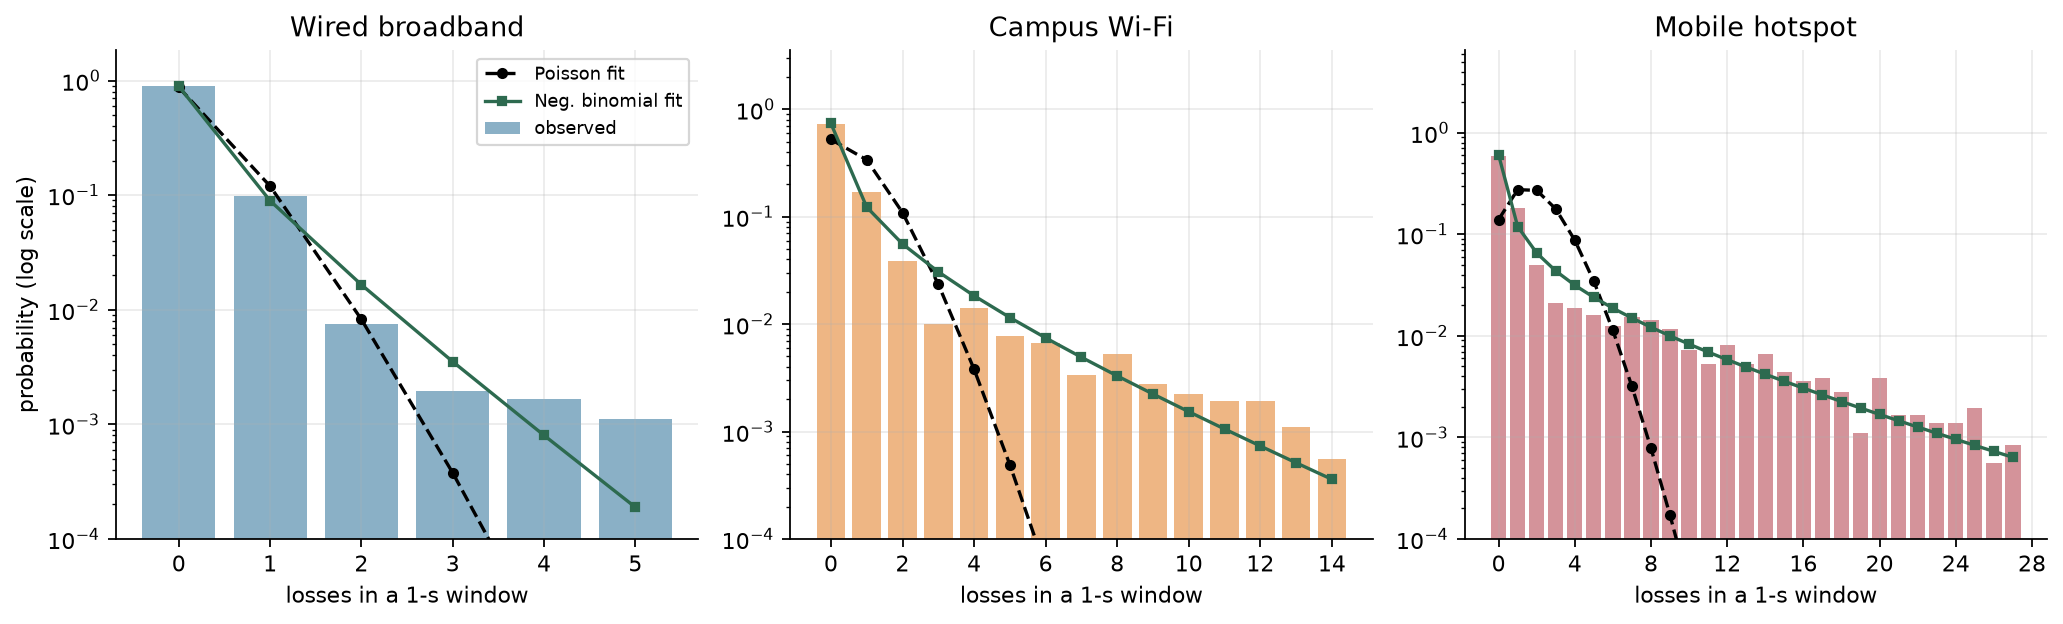
\includegraphics[width=\textwidth]{fig2_count_distribution_fits.png}
\caption{Probability of $k$ losses in one second, on a log scale. The Poisson fit (dashed) falls well below the observed tail, while the Negative Binomial (green) stays close to it.}
\label{fig:counts}
\end{figure*}

\subsection{Loss Counts}
None of the three networks fits the Poisson model, and Table~\ref{tab:counts} shows why. A Poisson distribution has its variance equal to its mean. The observed variance is <<list_D>> times the mean, and the dispersion test gives $p<10^{-10}$ in each case. The Negative Binomial fits much better and has a lower AIC on all three networks. The largest gain is on Mobile, where the AIC falls from <<M_aicP>> to <<M_aicNB>>.

Most of the difference between the two models lies in the tail. For Wi-Fi, the Poisson model expects about <<F_hpois>> seconds with <<heavy_k>> or more losses in an hour. The trace contains <<F_hobs>>, and the Negative Binomial expects <<F_hnb>>. Fig.~\ref{fig:counts} shows this on a log scale: the Poisson curve drops away almost at once, while the observed counts and the Negative Binomial carry on further out.

\begin{figure*}[!t]
\centering
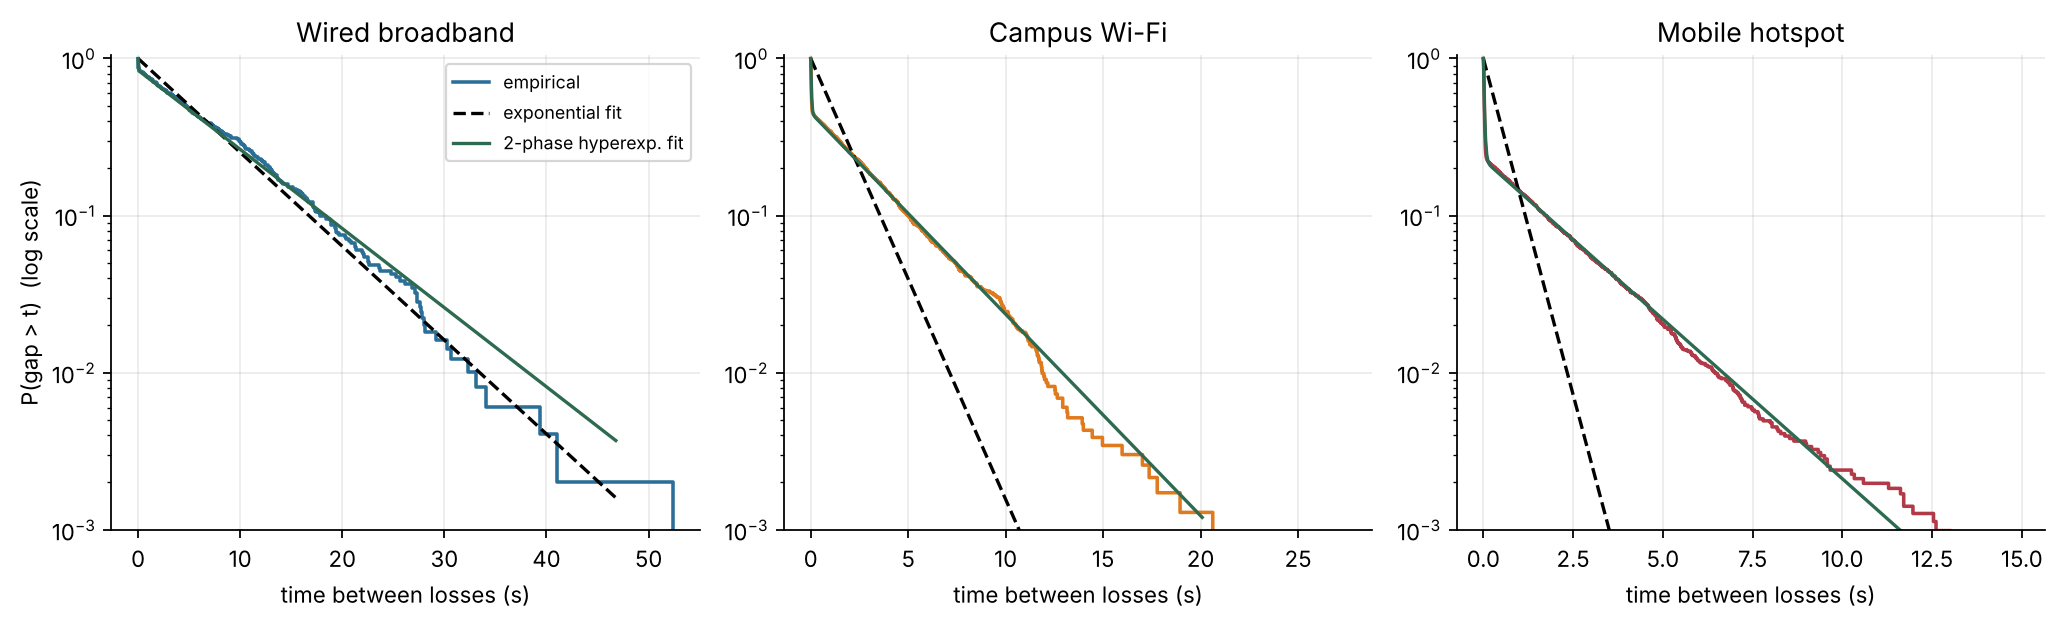
\includegraphics[width=\textwidth]{fig3_gap_survival.png}
\caption{Probability that the gap between two losses is longer than $t$, on a log scale. The exponential fit is a straight line (dashed); the two-phase mixture (green) bends with the data.}
\label{fig:gaps}
\end{figure*}

\begin{table*}[!t]
\caption{Losses per second and how well the count models fit}
\label{tab:counts}
\centering
\footnotesize
\setlength{\tabcolsep}{6pt}
\begin{tabular}{lcccccccc}
\toprule
Network & Loss rate & Mean / s & Variance & D & $\chi^2$ Poisson & AIC Poisson & AIC Neg. Bin. & Seconds with $\ge$<<heavy_k>> losses \\
\midrule
<<rows_counts>>
\bottomrule
\end{tabular}
\\[2pt]
\raggedright\scriptsize D is the variance divided by the mean. The last column gives the number of seconds with at least <<heavy_k>> losses: observed / expected under Poisson / expected under Negative Binomial. Every Poisson test gives $p<10^{-10}$.
\end{table*}

\subsection{Gaps Between Losses}
The exponential model is rejected as well, with the bootstrap KS test failing it on every network (Table~\ref{tab:gaps}). Fig.~\ref{fig:gaps} makes the problem easy to see. On a log scale an exponential survival curve is a straight line, and the observed curves are not straight. They fall steeply at first, because many of the gaps are very short, and then level off, because the remaining gaps are long.

The two-phase mixture reproduces this shape well. The mean gap in its fast phase is <<fast_lo>> to <<fast_hi>>~ms, one to two packets, which matches gaps inside a burst. The slow phase has a mean of <<M_slows>> to <<W_slows>>~s and matches the quiet periods between bursts. The share of gaps in the fast phase rises from <<W_wfast>> on Wired to <<M_wfast>> on Mobile, in line with more of the mobile link's losses falling inside bursts. The mixture passes the KS test on Wired ($p=<<W_ksmix>>$) and lowers the AIC considerably on all three networks. It is still rejected on Wi-Fi and Mobile, so it is a large improvement on the exponential but not a perfect description of the gaps.

\begin{table}[!t]
\caption{Gaps between losses: exponential and two-phase fits}
\label{tab:gaps}
\centering
\footnotesize
\setlength{\tabcolsep}{3pt}
\begin{tabular}{lccccccc}
\toprule
Net. & $w$ & Fast & Slow & \multicolumn{2}{c}{KS $p$} & \multicolumn{2}{c}{AIC} \\
 & & (ms) & (s) & exp. & mix. & exp. & mix. \\
\midrule
<<rows_gaps>>
\bottomrule
\end{tabular}
\\[2pt]
\raggedright\scriptsize $w$ is the share of gaps in the fast phase. Fast and slow are the average gap in each phase.
\end{table}

\subsection{Do Losses Depend on Each Other?}
They clearly do. Both independence tests reject $H_0$ with $p<10^{-10}$ on every network (Table~\ref{tab:dep}). For Wi-Fi we count <<F_runs>> runs, against about <<F_runsE>> expected under independence, a $z$-score of <<F_z>>. The Markov estimates make the effect easier to picture. On Wi-Fi a packet is lost <<F_a>> of the time when the packet before it was delivered, but <<F_b>> of the time when the packet before it was lost.

The posterior medians of $b/a$ are <<list_amp>> for Wired, Wi-Fi and Mobile, so a single loss makes the next loss <<amp_lo>> to <<amp_hi>> times more likely (Fig.~\ref{fig:markov}). The posterior probability that $b>a$ is <<pbga>> on every network, so the direction of the effect is not in doubt. The average bursts are short, at <<list_blen>> packets, but they happen far more often than they would by chance.

\begin{figure*}[!t]
\centering
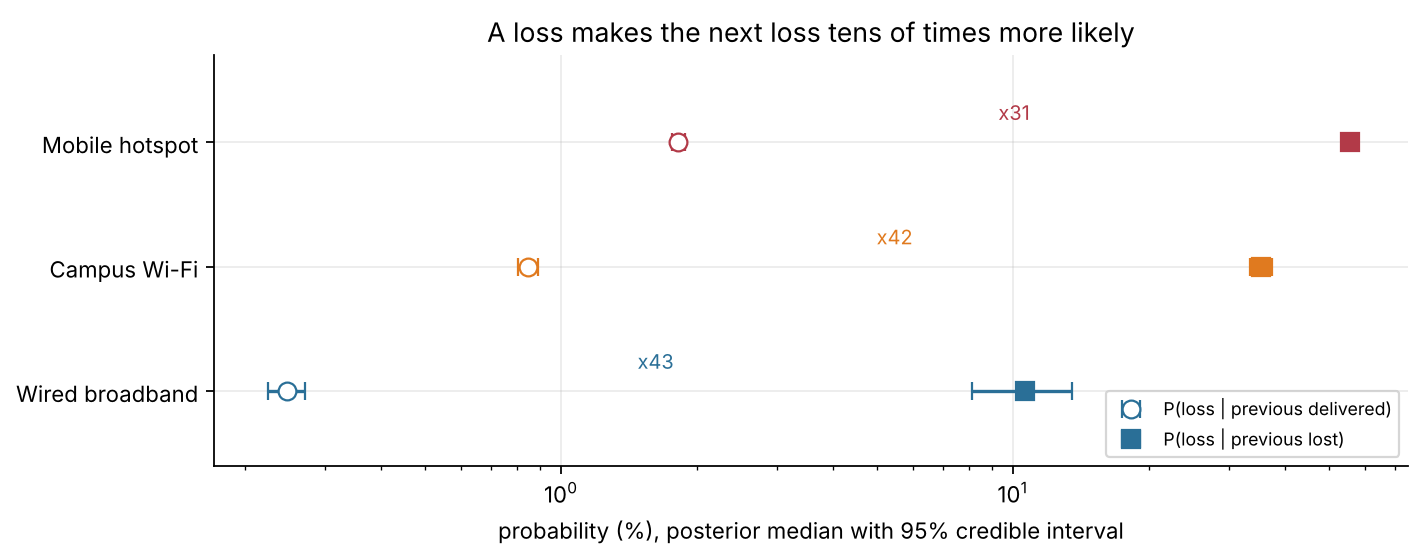
\includegraphics[width=0.72\textwidth]{fig5_markov_posteriors.png}
\caption{Posterior medians and 95\% credible intervals for $P(L\mid N)$ (open) and $P(L\mid L)$ (filled). On all three networks a loss sharply raises the chance that the next packet is lost too.}
\label{fig:markov}
\end{figure*}

\begin{table}[!t]
\caption{Tests of independence and burst parameters}
\label{tab:dep}
\centering
\footnotesize
\setlength{\tabcolsep}{2.2pt}
\begin{tabular}{lcccccccc}
\toprule
Net. & Runs & $E[R]$ & $z$ & $G^2$ & $P(L|N)$ & $P(L|L)$ & $b/a$ & Burst \\
\midrule
<<rows_dep>>
\bottomrule
\end{tabular}
\\[2pt]
\raggedright\scriptsize $b/a$ and burst length (in packets) are posterior medians. All $p<10^{-10}$.
\end{table}

\begin{figure*}[!t]
\centering
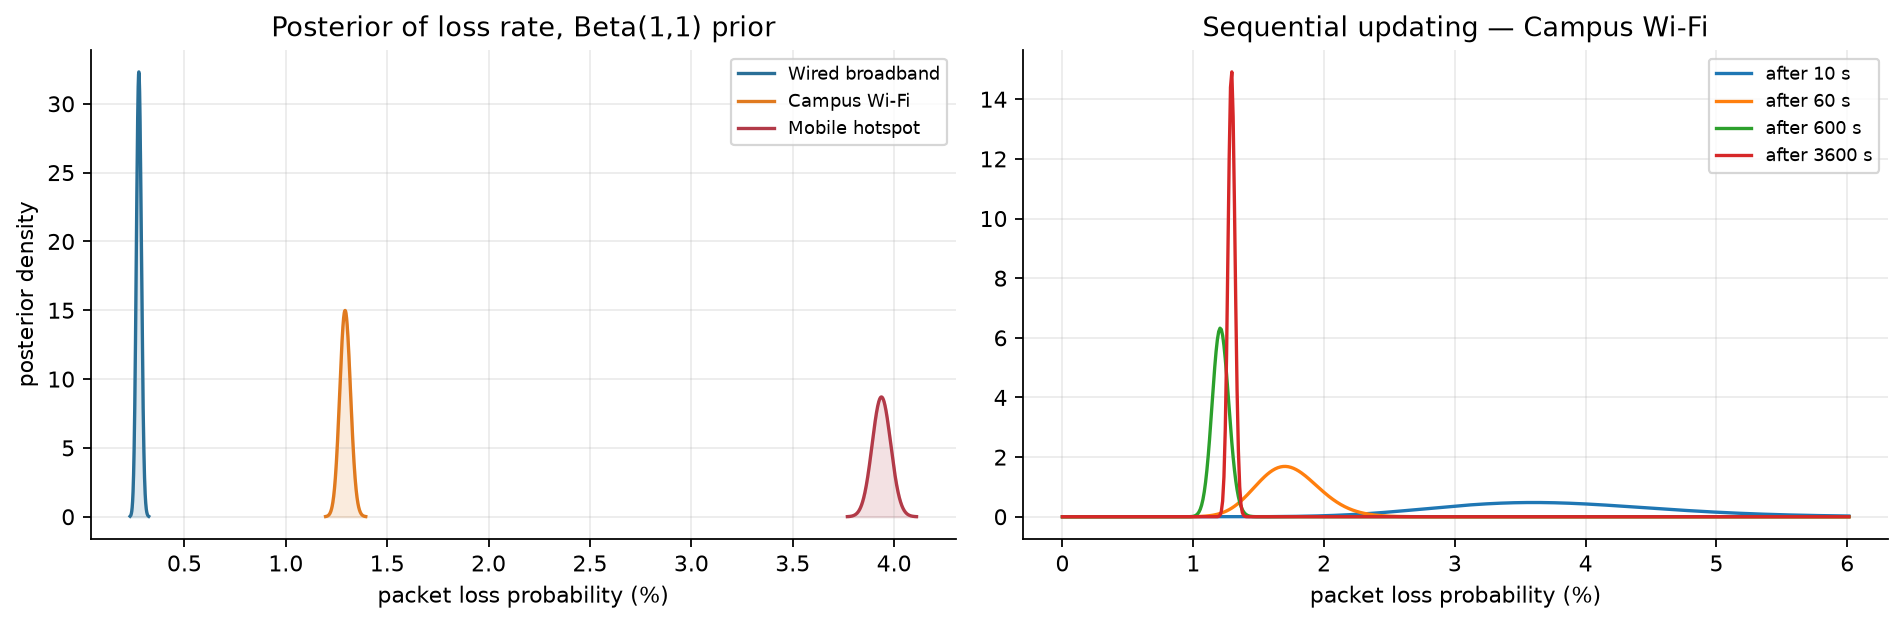
\includegraphics[width=\textwidth]{fig4_bayesian_posteriors.png}
\caption{Left: posterior distributions of the loss rate for the three networks. Right: the Wi-Fi posterior after 10~s, 60~s, 600~s and 3,600~s of traffic.}
\label{fig:bayes}
\end{figure*}

\subsection{Comparing the Networks}
The three networks differ clearly, as expected from how they were set up. The Kruskal-Wallis statistic is $H=<<kw_H>>$, the $\chi^2$ homogeneity statistic is <<chi_hom>> on <<chi_hom_df>> degrees of freedom, and even the largest Bonferroni-corrected pairwise p-value is <<bonf_max>>. The posterior mean loss rates are <<list_pmean>> (Table~\ref{tab:bayes}), and the posterior probability of the ordering Wired $<$ Wi-Fi $<$ Mobile is <<ordering>>.

Fig.~\ref{fig:bayes} shows the Bayesian estimates. With only <<seq_first_t>>~s of <<seq_label>> traffic the estimate is <<seq_first>>, a wide interval. After <<seq_last_t>>~s it has narrowed to <<seq_last>>.

The predictive check shows how poorly the independent model handles seconds with many losses. For Wi-Fi it puts the probability of a second with at least <<heavy_k>> losses at <<F_pred>>. In the trace such seconds make up <<F_seen>> of the total, about <<F_ratio>> times as often as predicted.

\subsection{How Often Do the Intervals Work?}
For us this is the key result. Across <<cov_reps>> simulated <<cov_min>>-minute captures, the naive 95\% interval included the true loss rate in only <<list_covN>> of cases (Table~\ref{tab:bayes}, Fig.~\ref{fig:coverage}). On the burstiest network it missed the true value more often than it caught it.

\begin{figure*}[!t]
\centering
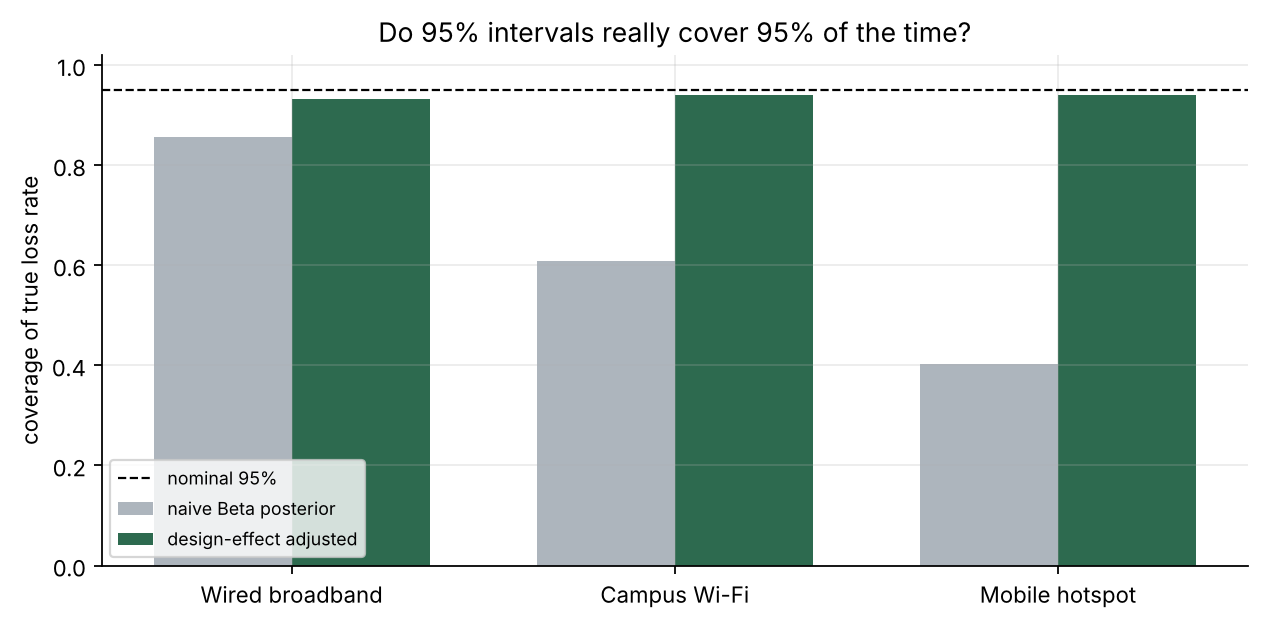
\includegraphics[width=0.62\textwidth]{fig7_interval_coverage.png}
\caption{Share of nominal 95\% intervals that contain the true loss rate, before and after the design-effect correction.}
\label{fig:coverage}
\end{figure*}

\begin{figure*}[!t]
\centering
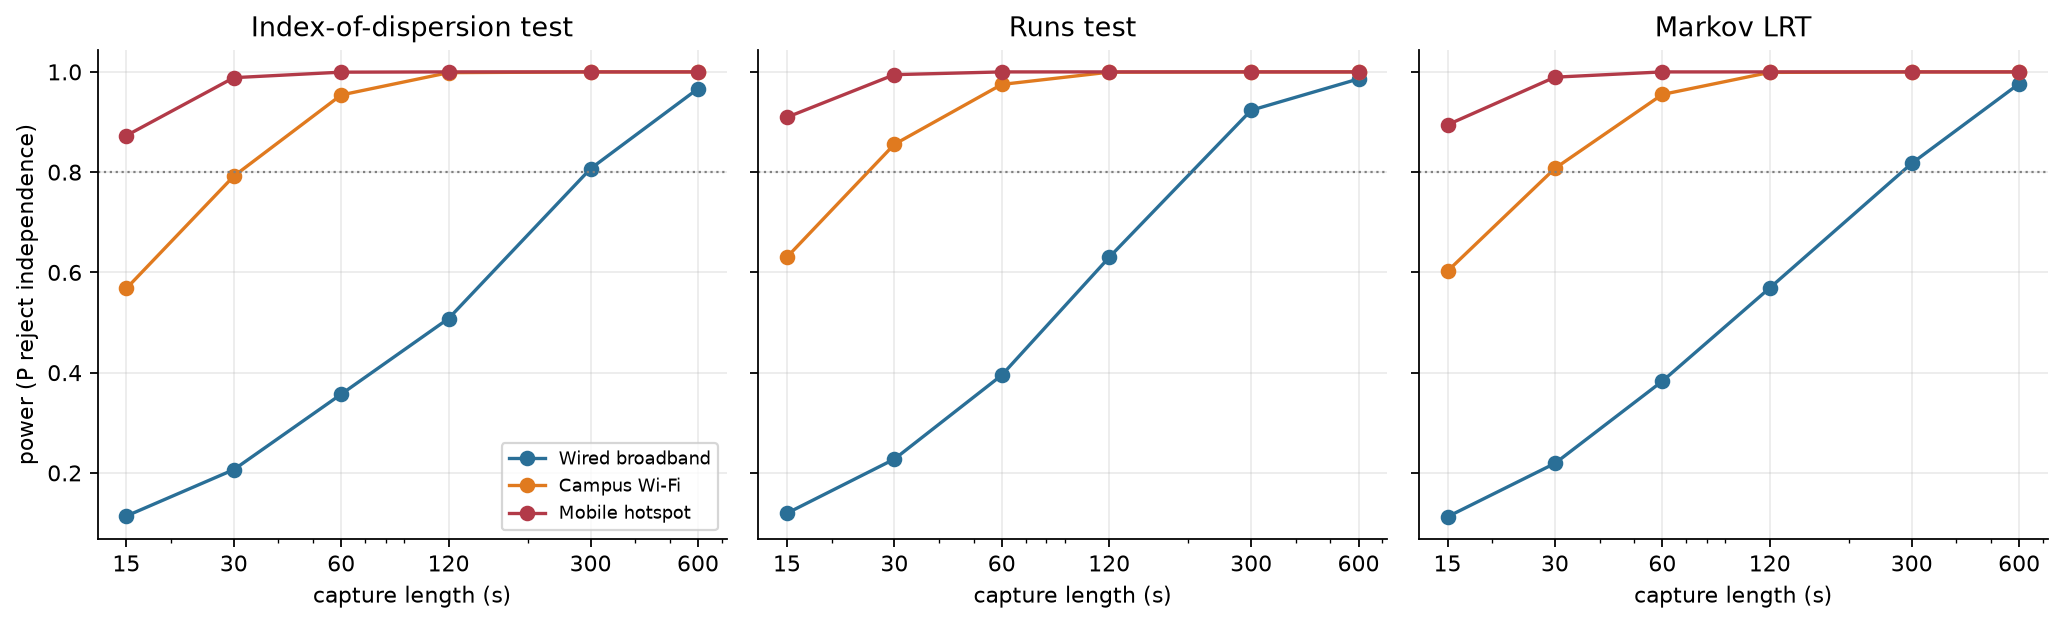
\includegraphics[width=\textwidth]{fig6_power_curves.png}
\caption{Power to detect dependence as capture length grows, from <<power_reps>> simulated captures per point. The dotted line marks a power of 0.8.}
\label{fig:power}
\end{figure*}

The design effects are <<W_deff>>, <<F_deff>> and <<M_deff>>. For Wi-Fi, this means our <<packets>> packets hold roughly the same information as <<F_neff>> independent packets would. With these smaller effective sample sizes, coverage returns to <<list_covA>>, close to the intended 95\%. The intervals do get wider; on Wi-Fi the average width grows from <<F_wN>> to <<F_wA>> percentage points. We think that is worth it for intervals that contain the true value about as often as they claim to.

The full Wi-Fi trace is a good example. Its true loss rate is <<F_true>>. The naive interval of <<F_pci>> lies entirely above this value, while the adjusted interval of <<F_aci>> contains it.

\begin{table*}[!t]
\caption{Loss-rate estimates and coverage of 95\% intervals}
\label{tab:bayes}
\centering
\footnotesize
\setlength{\tabcolsep}{8pt}
\begin{tabular}{lcccccc}
\toprule
Network & Posterior mean & Naive 95\% interval & deff & Adjusted 95\% interval & Naive coverage & Adjusted coverage \\
\midrule
<<rows_bayes>>
\bottomrule
\end{tabular}
\\[2pt]
\raggedright\scriptsize Intervals are from the full <<duration_h>>-hour trace. Coverage is from <<cov_reps>> simulated <<cov_min>>-minute captures.
\end{table*}

\subsection{How Long Should a Capture Be?}
Fig.~\ref{fig:power} shows how the power of each test increases with capture length, and Table~\ref{tab:power} lists the shortest length we tried at which power reaches <<power_target>>. With the runs test, the mobile network needs only <<M_pwR>>~s and Wi-Fi <<F_pwR>>~s. Wired needs <<W_pwR>>~s, since its bursts are infrequent and short and evidence takes longer to build up. The runs test was the most powerful of the three on every network. At <<dur_hi>>~s every test has a power of at least <<min_pw_hi>> on every network, which is why we plan to record at least ten minutes per network in Phase 2.

\section{Discussion and Limitations}
It takes surprisingly little for independence to fail. A Bad spell of only a few packets is enough to break every model built on that assumption, and the loss rate alone gives no hint of it. Mobile loses roughly <<ratio_MW>> times as many packets as Wired, yet on both networks a loss makes another loss tens of times more likely. Burstiness is a separate property of a link and has to be measured separately.

\begin{table}[!t]
\caption{Shortest capture (s) with power of at least <<power_target>>}
\label{tab:power}
\centering
\footnotesize
\begin{tabular}{lcccc}
\toprule
Network & Dispersion & Runs & Markov & Min. power at <<dur_hi>> s \\
\midrule
<<rows_power>>
\bottomrule
\end{tabular}
\end{table}

The coverage results show the problem is bigger than picking the right model. A naive interval counts every packet as a new and independent piece of evidence. When packets within a burst share the same outcome, there is much less independent evidence than the packet count suggests, and the interval turns out too narrow. The effect grows as the network becomes burstier, which is why Mobile has the lowest naive coverage. The design-effect correction is simple, needs only block counts, and brings coverage close to 95\% on all three networks.

Our conclusions are limited by certain factors. The data comes from the same model that motivated the study. True parameters were used only to judge the estimates, not by the tests. Some factors which are not accounted for by the model are: busy hours, moving users, and other traffic.

There are some additional points too. The dispersion test is a bit conservative as counts out of 50 are binomial, so the variance is just below the mean. This means that the test is more likely to underestimate burstiness than overestimate it. Runs and Markov tests use large-sample approximations which is fine for 1 hour traces. In very short captures their false-alarm rate may drift from 5\%, although for hour-long traces it stays close to 5\%. The Negative Binomial and the two-phase mixture are both still rejected on Wi-Fi and Mobile, so neither gives a complete description. The design effect depends on the block length we choose, and our <<block_s>>-s blocks are much longer than any Bad spell, which should be enough. Finally, the headline figures come from one seeded trace per network, although the Monte Carlo checks repeat the whole experiment thousands of times.

\section{Conclusion and Future Work}
We tested whether packet losses on <<n_scen>> simulated networks behave independently, and found that they do not. The Poisson and exponential models were rejected in every case. The per-second loss counts were <<list_D>> times more spread out than a Poisson model allows, the gaps split into short gaps within bursts and long quiet gaps between them, and each loss made the next one <<amp_lo>> to <<amp_hi>> times more likely. Most importantly, the standard 95\% interval for the loss rate was right in only <<covN_lo>> to <<covN_hi>> of cases. Dividing the sample size by the design effect raised this to between <<covA_lo>> and <<covA_hi>>.

The next step is Phase 2. We will record steady streams of <<rate>> packets per second on real wired, Wi-Fi and mobile links, for at least ten minutes each, and run the same code on them. After that we would like to estimate the Gilbert-Elliott parameters directly from the real traces using the Baum-Welch algorithm \cite{baum1970}, try richer models for the tail, use the Phase 1 results as priors in a hierarchical Bayesian model across the networks, and compare loss at peak and off-peak hours.

\section*{Reproducibility}
Every result in this report was produced by one Python pipeline, built on NumPy \cite{numpy2020}, SciPy \cite{scipy2020} and Matplotlib \cite{matplotlib2007} and run with seed <<seed>>. Running it again regenerates all of the tables and figures.

\begin{thebibliography}{99}
\bibitem{gilbert1960} E. N. Gilbert, ``Capacity of a burst-noise channel,'' \emph{Bell Syst. Tech. J.}, vol. 39, no. 5, pp. 1253-1265, 1960.
\bibitem{elliott1963} E. O. Elliott, ``Estimates of error rates for codes on burst-noise channels,'' \emph{Bell Syst. Tech. J.}, vol. 42, no. 5, pp. 1977-1997, 1963.
\bibitem{bolot1993} J.-C. Bolot, ``End-to-end packet delay and loss behavior in the Internet,'' in \emph{Proc. ACM SIGCOMM}, 1993, pp. 289-298.
\bibitem{paxson1997} V. Paxson, ``End-to-end Internet packet dynamics,'' in \emph{Proc. ACM SIGCOMM}, 1997, pp. 139-152.
\bibitem{yajnik1999} M. Yajnik, S. Moon, J. Kurose, and D. Towsley, ``Measurement and modelling of the temporal dependence in packet loss,'' in \emph{Proc. IEEE INFOCOM}, 1999, pp. 345-352.
\bibitem{jiang2000} W. Jiang and H. Schulzrinne, ``Modeling of packet loss and delay and their effect on real-time multimedia service quality,'' in \emph{Proc. NOSSDAV}, 2000.
\bibitem{hasslinger2008} G. Hasslinger and O. Hohlfeld, ``The Gilbert-Elliott model for packet loss in real time services on the Internet,'' in \emph{Proc. 14th GI/ITG Conf. Measurement, Modelling and Evaluation of Computer and Communication Systems (MMB)}, 2008, pp. 269-286.
\bibitem{dempster1977} A. P. Dempster, N. M. Laird, and D. B. Rubin, ``Maximum likelihood from incomplete data via the EM algorithm,'' \emph{J. Roy. Statist. Soc. B}, vol. 39, no. 1, pp. 1-38, 1977.
\bibitem{akaike1974} H. Akaike, ``A new look at the statistical model identification,'' \emph{IEEE Trans. Autom. Control}, vol. 19, no. 6, pp. 716-723, 1974.
\bibitem{lilliefors1969} H. W. Lilliefors, ``On the Kolmogorov-Smirnov test for the exponential distribution with mean unknown,'' \emph{J. Amer. Statist. Assoc.}, vol. 64, pp. 387-389, 1969.
\bibitem{efron1993} B. Efron and R. J. Tibshirani, \emph{An Introduction to the Bootstrap}. New York: Chapman \& Hall, 1993.
\bibitem{wald1940} A. Wald and J. Wolfowitz, ``On a test whether two samples are from the same population,'' \emph{Ann. Math. Statist.}, vol. 11, no. 2, pp. 147-162, 1940.
\bibitem{wilks1938} S. S. Wilks, ``The large-sample distribution of the likelihood ratio for testing composite hypotheses,'' \emph{Ann. Math. Statist.}, vol. 9, no. 1, pp. 60-62, 1938.
\bibitem{kruskal1952} W. H. Kruskal and W. A. Wallis, ``Use of ranks in one-criterion variance analysis,'' \emph{J. Amer. Statist. Assoc.}, vol. 47, pp. 583-621, 1952.
\bibitem{mann1947} H. B. Mann and D. R. Whitney, ``On a test of whether one of two random variables is stochastically larger than the other,'' \emph{Ann. Math. Statist.}, vol. 18, no. 1, pp. 50-60, 1947.
\bibitem{kish1965} L. Kish, \emph{Survey Sampling}. New York: Wiley, 1965.
\bibitem{gelman2013} A. Gelman, J. B. Carlin, H. S. Stern, D. B. Dunson, A. Vehtari, and D. B. Rubin, \emph{Bayesian Data Analysis}, 3rd ed. Boca Raton, FL: CRC Press, 2013.
\bibitem{baum1970} L. E. Baum, T. Petrie, G. Soules, and N. Weiss, ``A maximization technique occurring in the statistical analysis of probabilistic functions of Markov chains,'' \emph{Ann. Math. Statist.}, vol. 41, no. 1, pp. 164-171, 1970.
\bibitem{numpy2020} C. R. Harris \emph{et al.}, ``Array programming with NumPy,'' \emph{Nature}, vol. 585, pp. 357-362, 2020.
\bibitem{scipy2020} P. Virtanen \emph{et al.}, ``SciPy 1.0: Fundamental algorithms for scientific computing in Python,'' \emph{Nature Methods}, vol. 17, pp. 261-272, 2020.
\bibitem{matplotlib2007} J. D. Hunter, ``Matplotlib: A 2D graphics environment,'' \emph{Comput. Sci. Eng.}, vol. 9, no. 3, pp. 90-95, 2007.
\end{thebibliography}

\end{document}
